\documentclass[a4paper]{article}
\usepackage{amsmath}
\usepackage{graphicx}
\graphicspath{{../figures/}}



\begin{document}


\section*{SciML 2022 Exam}

This is the exam solution for Christian Michelsen in the Ph.D. course SciML 2022 at DTU.

\vspace{1cm}

\noindent The exam is based on the following sub-problems:
\begin{enumerate}
    \item Solve a damped harmonic oscillator with known parameters
    \item Generate data from the ODE solution
    \item Fit the data with a non-damped harmonic oscillator using a neural network to model the missing dynamics
    \item Try to symbolically recover the missing terms of the ODE (i.e. hopefully retrieve the original damped ODE)
    \item If time allows, fit the data from 2), but now with unknown parameters, using Turing and quantify the uncertainties
\end{enumerate}

\clearpage
\section*{1+2: Damped Harmonic Oscillator}

The damped harmonic oscillator (DHO) is, as the name suggests, a damped version of the classical harmonic oscillator (HO)
\begin{equation}
    m \ddot{x} + b\dot{x} + kx = 0.
    \label{eq:DHO}
\end{equation}
The dampening is determined by the damping parameter $b$, the mass is $m$, and the spring constant is $k$.
Here $\dot{x}$ refers to the first derivative of $x$ with respect to time $t$, and $\ddot{x}$ refers to the second derivative of $x$.
As such, the DHO is an differential equation governed by Newton's second law (the first term),
Hook's law (the last term) and the friction term (the second term).

Without loss of generality, we set $m=1$ and use unitless variables.
Equation \eqref{eq:DHO} can then be transformed to the following system:
\begin{equation}
    \begin{split}
        \dot{x} &= v \\
        \dot{v} &= -kx - bv.
    \end{split}
    \label{eq:DHO_2D}
\end{equation}

We solve \eqref{eq:DHO_2D} using \texttt{DifferentialEquations.jl} in Julia with the following parameters:
\begin{equation}
    \begin{split}
        b &= 0.1 \\
        k &= 0.1 \\
        x_0 &= 1.0 \\
        v_0 &= 1.0 \\
        t &\in [0, 40]
    \end{split}
\end{equation}
where $x_0$ and $v_0$ are the initial conditions for $x$ and $v$.
The solution to \eqref{eq:DHO} can be seen in Figure \ref{fig:DHO} as the solid, blue line.

\begin{figure}[htbp]
    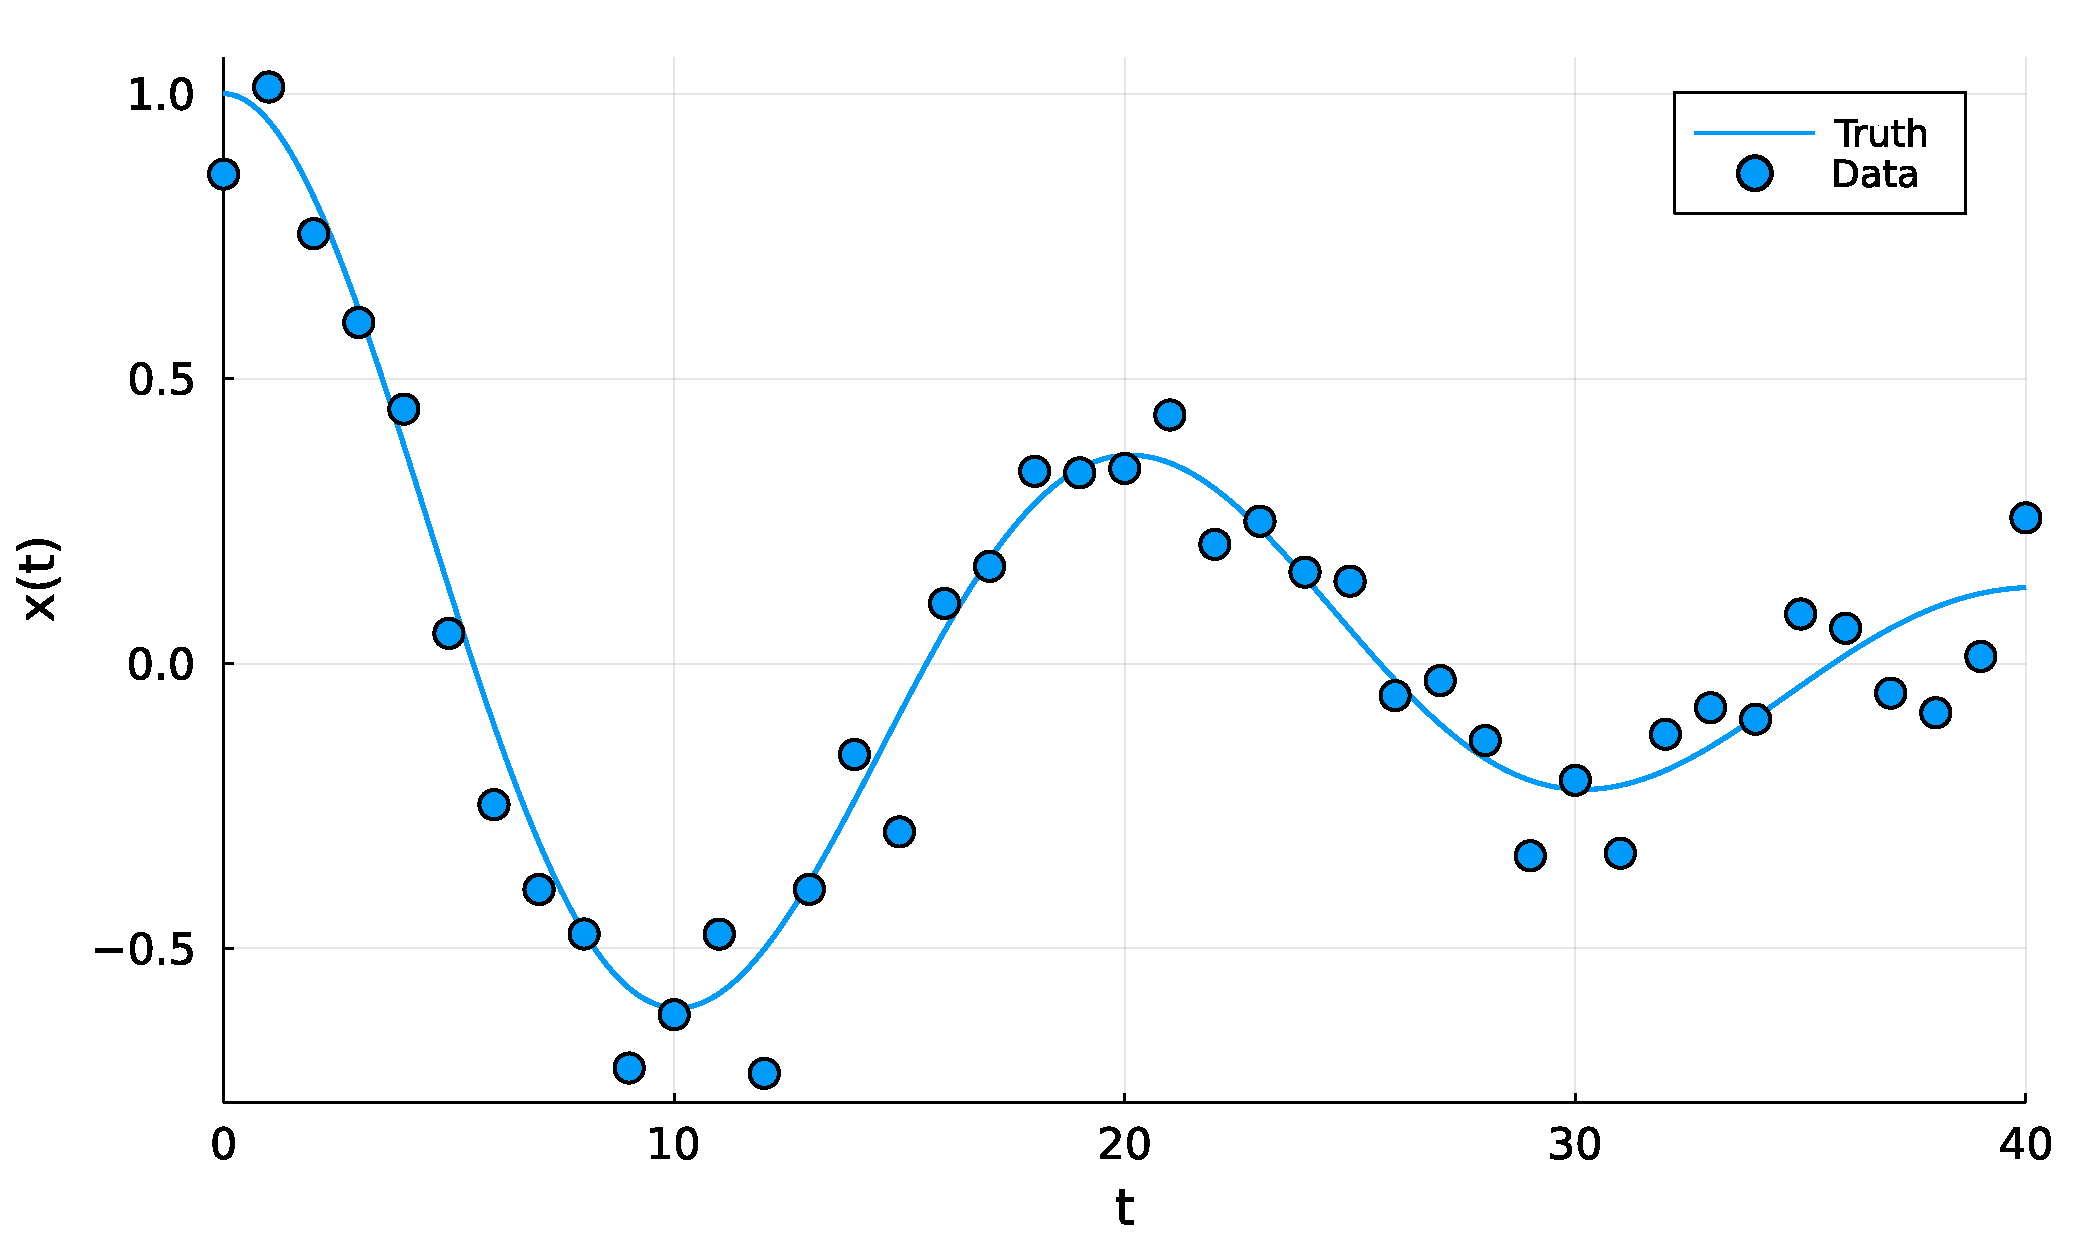
\includegraphics[width=\linewidth]{truth.pdf}
    \caption{The ODE solution is shown as the solid, blue line, and the simulated measurement data is shown as blue points.}
    \label{fig:DHO}
\end{figure}

We generate data from the ODE solution by taking equidistant time steps between $0$ and $40$ such that $\Delta t = 1.0$.
On top of this, we add some noise to the data to simulate measurement noise.
The blue points in Figure \ref{fig:DHO} are the data (including noise).


\end{document}